\begin{enumerate}
\item \lstinputlisting[style=Matlab-editor,basicstyle=\mlttfamily,title=\lstname]{progs/matlab/matrixAlgebraEigenvalues.m}
In the univariate AR(1) model we would check whether the autocorrelation coefficient is between -1 and 1,
  i.e.\ whether \(|\phi| = |A|<1\) such that \(\sum_{j=0}^\infty (AL)^j=1/(1-AL)\) where \(L\) is the lag operator.
In the multivariate case, we want to check the same thing,
  i.e. \(\sum_{j=0}^\infty (AL)^j=(1-AL)^{-1}\).
Note that \(A\) is a square matrix and taking the power of a matrix is not a trivial task.
One convenient way to do so, is to consider an eigenvalue decomposition (if it exists):
\[A= Q \Lambda Q^{-1}\]
  where \(Q\) is a square matrix whose columns contain the eigenvectors \(q_i\)
  corresponding to the eigenvalues \(\lambda_i\) found on the diagonal of \(\Lambda = {[\lambda_i]}_{ii}\).
Moreover, \(\Lambda \) is a diagonal matrix and \(Q\) is an orthogonal matrix \(Q^{-1}=Q'\).
Using this decomposition one can show that it is very easy to compute any power of a matrix:
\begin{itemize}
    \item matrix inverse \(A^{-1} = Q \Lambda^{-1} Q^{-1}\) where the inverse of \([\Lambda^{-1}]_{ii} = 1/\lambda_i\) is very easy to calculate as it is a diagonal matrix
    \item matrix powers: \(A^2=(Q\Lambda Q^{-1})(Q\Lambda Q^{-1})=Q\Lambda (Q^{-1}Q) \Lambda Q^{-1} = Q \Lambda^2 Q^{-1}\) or more generally: \(A^j = Q \Lambda^j Q^{-1}\).
\end{itemize}
So, for \(\sum_{j=0}^\infty {(AL)}^j=(1-AL)^{-1}\) we need that \(\lim_{j\rightarrow \infty}\Lambda^j=0\).
As this is a diagonal matrix, the task simplifies as we only need to look at each eigenvalue whether it is between -1 and 1: \(|\lambda_i|<1\).
In other words, for VAR(1) systems \(y_t = c + A y_{t-1} + u_t\) we need to check whether the eigenvalues of \(A\) are inside the unit circle.
If they are, then the VAR(1) model is said to be both stable and covariance-stationary.
	
\item Example for vectorization and Kronecker product:
\begin{align*}
    \underbrace{vec\begin{pmatrix} 1&3&2\\1&0&0\\1&2&2 \end{pmatrix}}_{3\times3} = \underbrace{\begin{pmatrix} 1 \\1 \\1 \\3 \\0 \\2 \\2 \\ 0 \\2\end{pmatrix}}_{9\times1}, \qquad 
    \underbrace{\begin{pmatrix} 1&3&2\\1&0&0\\1&2&2 \end{pmatrix}}_{3\times3} \otimes \underbrace{\begin{pmatrix}0&5\\5&0\\1&1 \end{pmatrix}}_{3\times2} =
    \underbrace{\begin{pmatrix} 1\cdot\begin{pmatrix}0&5\\5&0\\1&1 \end{pmatrix}&3\cdot\begin{pmatrix}0&5\\5&0\\1&1 \end{pmatrix}&2\cdot\begin{pmatrix}0&5\\5&0\\1&1 \end{pmatrix}\\1\cdot\begin{pmatrix}0&5\\5&0\\1&1 \end{pmatrix}&0\cdot\begin{pmatrix}0&5\\5&0\\1&1 \end{pmatrix}&0\cdot\begin{pmatrix}0&5\\5&0\\1&1 \end{pmatrix}\\1\cdot\begin{pmatrix}0&5\\5&0\\1&1 \end{pmatrix}&2\cdot\begin{pmatrix}0&5\\5&0\\1&1 \end{pmatrix}&2\cdot\begin{pmatrix}0&5\\5&0\\1&1 \end{pmatrix}  \end{pmatrix}}_{9\times6}
\end{align*}
Using this definition, we can show that \(vec(DEF) = (F' \otimes D) vec(E)\) using e.g.\ a symbolic toolbox:
\lstinputlisting[style=Matlab-editor,basicstyle=\mlttfamily,title=\lstname]{progs/matlab/matrixAlgebraKroneckerFormula.m}
Of course you can do this on paper as well:		 
\begin{align*}
DEF &= D \begin{pmatrix} e_1 & e_2 & \cdots & e_p \end{pmatrix}
\begin{pmatrix}
f_{11} &f_{12} &\cdots &f_{1k} \\
f_{21} &f_{22} &\cdots &f_{2k} \\
\vdots &\vdots &\vdots &\vdots\\
f_{p1} &f_{p2} &\cdots &f_{pk}
\end{pmatrix}\\
&= D \underbrace{\begin{pmatrix} e_1f_{11}+e_2f_{21}+\cdots+e_p f_{p1},& e_1f_{12}+e_2f_{22}+\cdots+e_p f_{p2}, & \dots ,& e_1f_{1k}+e_2f_{2k}+\cdots+e_p f_{pk}\end{pmatrix}}_{n\times k}
\end{align*}
Vectorizing:
\begin{align*}
vec(DEF) &= \begin{pmatrix} f_{11}D e_1 +f_{21}D e_2+\cdots+ f_{p1}D e_p\\ f_{12}D e_1+f_{22} D e_2 + \cdots +  f_{p2} D e_p \\ \vdots \\ f_{1k} D e_1+ f_{2k} D e_2 +\cdots+ f_{pk} D e_p  \end{pmatrix}
= \begin{pmatrix} f_{11}D &  f_{21}D  & \cdots & f_{p1}D \\ f_{12}D  & f_{22} D & \cdots & f_{p2} D\\ \vdots & \vdots &\vdots&\vdots \\ f_{1k}D & f_{2k} D &\cdots& f_{pk} D  \end{pmatrix} \begin{pmatrix} e_1\\e_2\\ \vdots \\ e_p\end{pmatrix}\\
&= \left(F'\otimes D\right) vec(E)
\end{align*}

\item An orthogonal matrix is characterized by \(R'=R^{-1}\) and therefore \(R'R=R R' = I\).
Here:
\begin{align*}
R'R = \begin{pmatrix}
(\cos(\phi))^2 + (\sin(\phi))^2 & -\cos(\phi)\sin(\phi) + \sin(\phi)\cos(\phi)\\-\sin(\phi)\cos(\phi) + \cos(\phi)\sin(\phi) & (\sin(\phi))^2 + (\cos(\phi))^2
\end{pmatrix}
\end{align*}
with \((\cos(\phi))^2 + (\sin(\phi))^2 = 1\) (so-called trigonometric Pythagoras).
		 
\lstinputlisting[style=Matlab-editor,basicstyle=\mlttfamily,title=\lstname]{progs/matlab/matrixAlgebraRotation.m}
		 
\(R\) is called a rotation matrix,
  because it rotates vectors or objects in the Euclidian space without stretching or shrinking the object.
\begin{center}  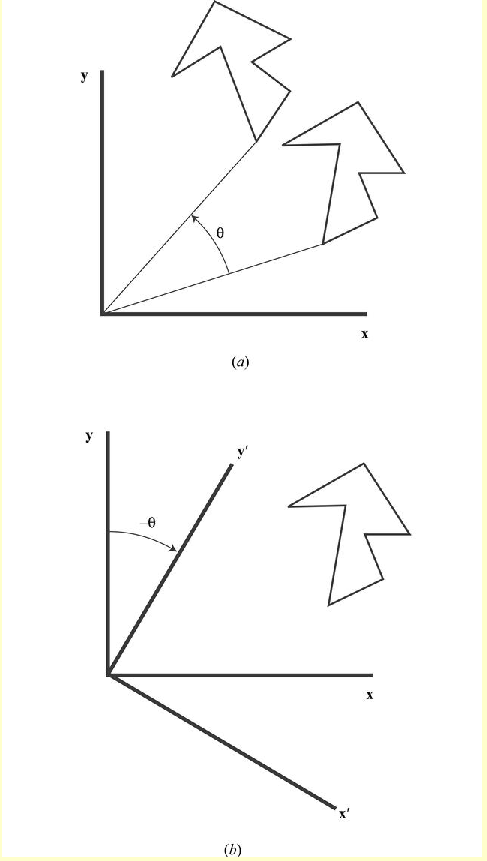
\includegraphics[width=.5\textwidth]{plots/Rotation.png} \end{center}
In this example the matrix R rotates the vector counter-clockwise given angle \(\phi\).
An active rotation means that the vector is multiplied by the rotation matrix and this rotates the vector counterclockwise \(x' = Rx\).
A passive rotation means that the coordinate system is rotated and therefore the vector is also rotated: \(x' = R^{-1} x\).
Later on we will need rotation matrices for identification of structural shocks!

\item \lstinputlisting[style=Matlab-editor,basicstyle=\mlttfamily,title=\lstname]{progs/matlab/matrixAlgebraCholesky.m}
\begin{align*}
\underbrace{\begin{pmatrix}1&0&0\\0&1&0\\0&0.5&1\end{pmatrix}}_W \underbrace{\begin{pmatrix}2.25&0&0\\0&1&0\\0&0&0.49\end{pmatrix}}_{\Sigma_\varepsilon} \underbrace{\begin{pmatrix}1&0&0\\0&1&0.5\\0&0&1\end{pmatrix}}_{W'} = \underbrace{\begin{pmatrix}2.25&0&0\\0&1&0.5\\0&0.5&0.74\end{pmatrix}}_{\Sigma}
\end{align*}

\item Solving this equation can be done either analytically or using an algorithm:
\begin{enumerate}
    \item Analytically:
        \begin{align*}
            vec(\Sigma_y) &= vec(A \Sigma_y A') + vec(\Sigma_u) = (A \otimes A)vec(\Sigma_y) + vec(\Sigma_u)\\
            (I-A\otimes A)vec(\Sigma_y) &= vec(\Sigma_u)\\
            vec(\Sigma_y) &= (I-A\otimes A)^{-1}vec(\Sigma_u)
        \end{align*}
    \item Doubling algorithm:
    \lstinputlisting[style=Matlab-editor,basicstyle=\mlttfamily,title=\lstname]{progs/matlab/dlyapdoubling.m}
    The basic idea of the doubling algorithm is to start at some \(\Sigma_{y,0}\)
    and find new values for \(\Sigma_{y,i+1}\) using the equation \(A \Sigma_{y,i} A' + \Sigma_u\)
    until the difference \(\Sigma_{y,i+1} - \Sigma_{y,i}\) becomes very small
    or a certain maximum number of iterations is reached.
    
    The doubling algorithm, however, allows one to pass in one iteration
    from \(\Sigma_{y,i}\) to \(\Sigma_{y,2i}\) rather than \(\Sigma_{y,i+1}\),
    provided that one updates three other matrices.
    There are also other (generalized) algorithms to solve such matrix Lyapunov (or Sylvester) equations.

    \item Comparison:
    \lstinputlisting[style=Matlab-editor,basicstyle=\mlttfamily,title=\lstname]{progs/matlab/matrixAlgebraLyapunovComparison.m}
    The doubling algorithm is faster than the analytical closed-form expression based on the Kronecker product.
\end{enumerate}
		
\end{enumerate}